
\section[伙伴算法简易实现]{伙伴算法简易实现}
\begin{center}
  % Requires \usepackage{graphicx}
  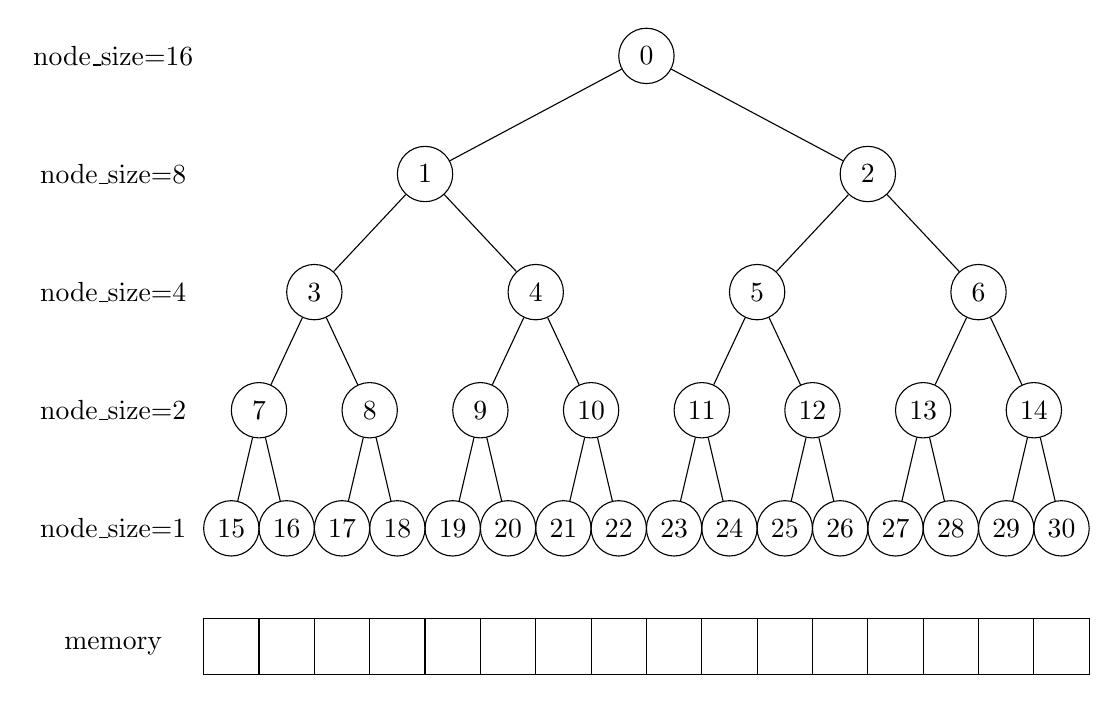
\begin{tikzpicture}
  [every node/.style={minimum size=20pt, inner sep=2pt},
   tree-node/.style={draw,circle},
   side-node/.style={},
   memo-node/.style={draw,rectangle},
   level 1/.style={sibling distance=160pt}, % 8 * 20pt
   level 2/.style={sibling distance=80pt}, % 4 * 20pt
   level 3/.style={sibling distance=40pt}, % 2 * 20pt
   level 4/.style={sibling distance=20pt}] % 1 * 20pt
  \node [tree-node] (root) {0}
    child {
      node [tree-node] {1}
        child {
          node [tree-node] {3}
            child {
              node [tree-node] {7}
                child {
                  node [tree-node] {15}
                    child [grow=down] {
                      node [memo-node] {} edge from parent[draw=none]
                        child [grow=left] {node [side-node] {memory} edge from parent[draw=none]}
                    }
                    child [grow=left] {
                      node [side-node] {node\_size=1} edge from parent[draw=none]
                        child [grow=up] {
                          node [side-node] {node\_size=2} edge from parent[draw=none]
                            child [grow=up] {
                              node [side-node] {node\_size=4} edge from parent[draw=none]
                                child [grow=up] {
                                  node [side-node] {node\_size=8} edge from parent[draw=none]
                                    child [grow=up] {
                                      node [side-node] {node\_size=16} edge from parent[draw=none]
                                    }
                                }
                            }
                        }
                    }
                }
                child {
                  node [tree-node] {16}
                    child [grow=down] {node [memo-node] {} edge from parent[draw=none]}
                }
            }
            child {
              node [tree-node] {8}
                child {
                  node [tree-node] {17}
                    child [grow=down] {node [memo-node] {} edge from parent[draw=none]}
                }
                child {
                  node [tree-node] {18}
                    child [grow=down] {node [memo-node] {} edge from parent[draw=none]}
                }
            }
        }
        child {
          node [tree-node] {4}
            child {
              node [tree-node] {9}
                child {
                  node [tree-node] {19}
                    child [grow=down] {node [memo-node] {} edge from parent[draw=none]}
                }
                child {
                  node [tree-node] {20}
                    child [grow=down] {node [memo-node] {} edge from parent[draw=none]}
                }
            }
            child {
              node [tree-node] {10}
                child {
                  node [tree-node] {21}
                    child [grow=down] {node [memo-node] {} edge from parent[draw=none]}
                }
                child {
                  node [tree-node] {22}
                    child [grow=down] {node [memo-node] {} edge from parent[draw=none]}
                }
            }
        }
    }
    child {
      node [tree-node] {2}
        child {
          node [tree-node] {5}
            child {
              node [tree-node] {11}
                child {
                  node [tree-node] {23}
                    child [grow=down] {node [memo-node] {} edge from parent[draw=none]}
                }
                child {
                  node [tree-node] {24}
                    child [grow=down] {node [memo-node] {} edge from parent[draw=none]}
                }
            }
            child {
              node [tree-node] {12}
                child {
                  node [tree-node] {25}
                    child [grow=down] {node [memo-node] {} edge from parent[draw=none]}
                }
                child {
                  node [tree-node] {26}
                    child [grow=down] {node [memo-node] {} edge from parent[draw=none]}
                }
            }
        }
        child {
          node [tree-node] {6}
            child {
              node [tree-node] {13}
                child {
                  node [tree-node] {27}
                    child [grow=down] {node [memo-node] {} edge from parent[draw=none]}
                }
                child {
                  node [tree-node] {28}
                    child [grow=down] {node [memo-node] {} edge from parent[draw=none]}
                }
            }
            child {
              node [tree-node] {14}
                child {
                  node [tree-node] {29}
                    child [grow=down] {node [memo-node] {} edge from parent[draw=none]}
                }
                child {
                  node [tree-node] {30}
                    child [grow=down] {node [memo-node] {} edge from parent[draw=none]}
                }
            }
        }
    };
\end{tikzpicture}
  %\caption{buddy system}\label{fig:buddy}
\end{center}


从伙伴算法看满二叉树的一些特性:
\begin{description}
  \item[total\_leaf\_size] 满二叉树的叶子节点总数
  \item[level] 满二叉树的层级,范围0-max\_depth
  \item[node\_size] 每个level上节点的size
  \item[index] 某个节点在满二叉树数组中的索引
  \item[offset] 某一个节点对应的内存单元映射到叶子节点数组中的下标(offset)
\end{description}
total\_leaf\_size是已知的,即buddy system管理的内存单元总数。
$$ max\_depth = \log_2total\_leaf\_size$$
每个level上第一个左子树的index为$2^{level} - 1$
\begin{align*}
  offset & = [index - (2^{level} - 1)] * node\_size \\
         & = (index + 1) * node\_size - 2^{level} * node\_size \\
         & = (index + 1) * node\_size - 2^{level} * 2^{max\_depth - level} \\
         & = (index + 1) * node\_size - 2^{max\_depth} \\
         & = (index + 1) * node\_size - total\_leaf\_size \\
\end{align*}
可见,无论哪个level,第一个左子树(最左边的节点)对应到叶子节点数组中的下标总是0.